\chapter{Funktionstest/Validierung}\label{chap:Funktionstest}
\thispagestyle{standard}
\pagestyle{standard}
\lfoot{\small Markus Haas}

\section{Virtual Machine Management}
\label{sec:VirtualMachineManagement}
Zum Testen des Protokolladapters ist ein Netzwerk von \acl{VM}s (\acs{VM}s) eingerichtet worden. Als Virtualisierungssoftware wurde Virtualbox 5.1\footnote{\url{https://www.virtualbox.org/}} von Oracle verwendet. Genauere Informationen zur VM sind in der Tabelle \ref{tab:OverviewVM} enthalten. Als nächster Schritt folgte die Installation der Entwicklungsumgebung Eclipse. Abbildung \ref{fig:NetworkOverview} zeigt eine Übersicht des eingerichteten Netzwerks. Dabei agiert eine VM als Modbus Client und zwei weitere VMs sind Modbus Server. Um die in Kapitel \ref{sec:PushFunction} beschriebene Funktion \grqq{}Push 1:n\grqq{} zu simulieren sind mehrere Server notwendig. Die VMs sind über das interne Netzwerk verbunden, welches von Virtualbox bereitgestellt wird. 

\begin{figure}[h]
	\centering
	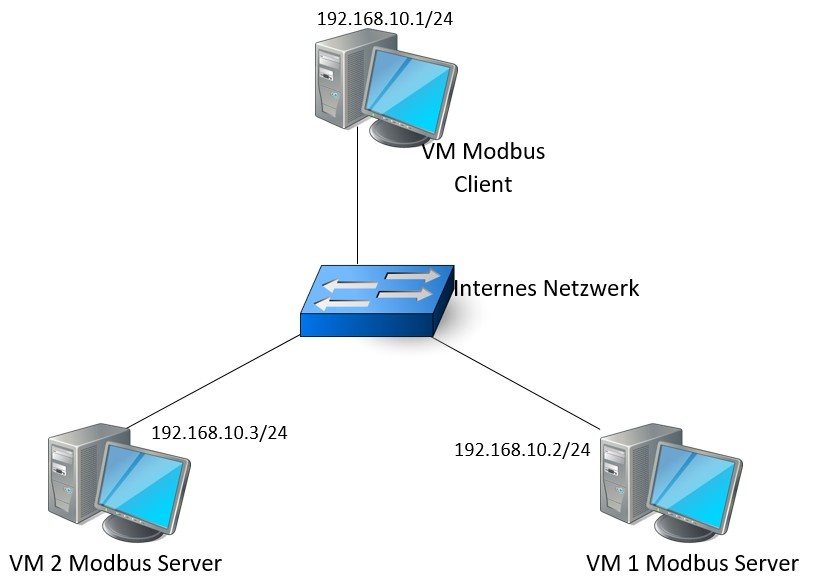
\includegraphics[width=10cm]{BilderAllgemein/Netzwerkuebersicht.jpg}\medskip
	\caption{Netzwerkübersicht}
	\label{fig:NetworkOverview}
\end{figure}


\begin{table}[h]
\centering
\begin{tabular}{|l|c|c|c|}
\hline
                         & Client                 & Server 1              & Server 2              \\ \hline
IP V4 Adresse            & 192.168.10.1/24        & 192.168.10.2/24       & 192.168.10.3/24       \\ \hline
OS                       & \multicolumn{3}{c|}{Windows 7 Ultimate 64 bit V6.1.7601 SP1 Build 7601} \\ \hline
RAM                      & \multicolumn{3}{c|}{2048Mb}                                            \\ \hline
CPUs                     & \multicolumn{3}{c|}{4 paravirtualisiert}                               \\ \hline
Virtualisierungssoftware & \multicolumn{3}{c|}{Virtual Box 5.1.12 r112440}                        \\ \hline
\end{tabular}
\caption{Übersicht VMs}
\label{tab:OverviewVM}
\end{table}

\section{Ausgangsbedingungen und Abgrenzungen}
Als Testumgebung wurde die bereits in Kapitel \ref{sec:VirtualMachineManagement} beschriebene Konfiguration verwendet. Auf der Client VM sind die Pakete mit dem Programm Wireshark\footnote{\url{https://www.wireshark.org/}} aufgezeichnet worden. Zur besseren Übersicht sind  die Daten des TCP Segments welche für Modbus relevant sind in Tabellenform dargestellt. Die Publish-Subscribe Funktion wird nicht separat behandelt, da diese der Grundfunktion der Request-Response Funktion entspricht.


\subsection{Modbus Server}
Zum Testen der Funktionen des Protokolladapters werden zwei Modbus Server verwendet. Programmiert wurden diese unter der Verwendung der Java Library Modbus4j. SunSpec lässt verschiedene Informationsmodelle zu. Zum Testen wurde das in \cite{ModbusSunSpecFronius} auf den Seiten 25 bis 29 angegebene Modell implementiert. Im ersten Schritt wurden die im Dokument beschriebenen Register erzeugt und mit zufälligen Werten initialisiert. Das Objekt in welchem sich die Register befinden ist vom Typ \textit{BasicProcessImage}. Beim Erzeugen des Objekts muss die Modbus Slave ID übergeben werden. Somit können auf einem Server mehrere Objekte vom Typ \textit{BasicProcessImage} erzeugt werden. Die unterschiedlichen Objekte werden von einem Client über die Slave ID des Modbus Protokolls angesprochen. Bei Modbus TCP ist ein Server über die IP-Adresse und Slave ID eindeutig identifizierbar. Ein Modbus TCP Gerät kann deshalb mehrere Modbus Server bereitstellen. Es ist das Gateway zu mehreren Modbus Servern. Ein \textit{BasicProcessImage} Objekt dient zum  Austausch der Daten zwischen Modbus Server und der Applikation welche am Server läuft. Nach der Erzeugung des Prozessabbildes wird der Modbus Server in einem Thread gestartet. Parallel dazu wird ein weiterer Thread gestartet. Dem Programm im zweiten Thread wird die Referenz des \textit{BasicProcessImage} Objekts übergeben. Das Programm in diesem Thread springt in eine Endlosschleife und gibt die Werte der Register in der Kommandozeile aus. Bei statischen Werten ist es nicht möglich, die Funktion Publish-Subscribe zu testen. Deshalb ändert dieses Programm die Werte in den Registern. Nach dem Durchlauf des Programms wird der Thread für eine Zeit pausiert.
\clearpage


\section{Push1-N (send)}

In diesem Kapitel wird der Test zum Validieren der implementierten Push1-N Funktion beschrieben.

\subsection{Ausgangssituation}
\label{sec:PushAusgangssituation}
Auf VM1 ist ein Modbus Server eingerichtet. Im Bild \ref{fig:PushBeforeModbusServerVM1} ist dargestellt, wie die Applikation zyklisch den SunSpec Float Wert ab Registeradresse 40072 ausgibt.

\begin{figure}[h]
	\centering
	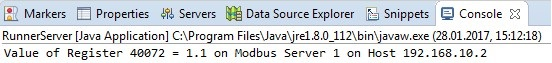
\includegraphics[width=14cm]{BilderAllgemein/pushServer1Ausgang.jpg}\medskip
 	\caption{Modbus Server VM1 vor dem Test}
 	\label{fig:PushBeforeModbusServerVM1}
\end{figure}

Auf VM2 sind zwei Modbus Server eingerichtet. Im Bild \ref{fig:PushBeforeModbusServerVM2} ist dargestellt, wie die Applikation zyklisch den SunSpec Float Wert ab Registeradresse 40072 der beiden Modbus Server ausgibt.

\begin{figure}[h]
	\centering
	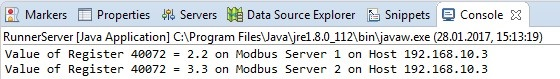
\includegraphics[width=14cm]{BilderAllgemein/pushServer2Ausgang.jpg}\medskip
 	\caption{Modbus Server VM2 vor dem Test}
 	\label{fig:PushBeforeModbusServerVM2}
\end{figure}

Angemerkt sei, dass alle 3 Register vor dem Test einen unterschiedlichen Wert besitzen.

\subsection{Test}
Mit der \textit{send} Methode der \textit{ModbusTCPAdapter} Klasse wird nun ein Wert an die im Kapitel \ref{sec:PushAusgangssituation} beschriebenen Server gesendet. Listing \ref{lst:send} zeigt den Methodenaufruf. Dabei wird eine Liste mit der \textit{Remoteaddress} der 3 Modbus Server erzeugt. Ebenfalls wird eine Liste an \textit{Status} Objekten erzeugt. Geschrieben soll der Wert 10.0 im SunSpec \textit{Float} Format werden. Nach dem Aufruf der Methode werden die Rückgabeobjekte der Methode zu Testzwecken auf die Kommandozeile geschrieben. Im folgenden Abschnitt wird, stellvertretend für alle Transaktionen, nur eine Transaktion zu einem Server betrachtet. Prinzipiell funktionieren die Transaktionen gleich.
\clearpage


\lstset{language=Java, numbers=left, numberstyle=\tiny, stepnumber=2, numbersep=5pt, tabsize=2}
\begin{lstlisting}[caption={Methodenaufruf send},label=lst:send, xleftmargin=50pt]
public static void main(String[] args){
	//Neuer Adapter 
	ModbusTCPAdapter Adapter = ModbusTCPAdapter.getInstanz();
	
	// Liste von Verbindungen
	List<String> ConnectionParameter = new LinkedList<>();
	//Liste fuer Rueckmeldungen
	List<Status> FeedbackStatus = new LinkedList<>();
	
	//Wert zuweisen
	DataObject value = new DataObject();
	value.data = 10.0;
		
	//Modbus Server hinzufuegen
	ConnectionParameter.add("192.168.10.2:1:40072:float32");
	ConnectionParameter.add("192.168.10.3:1:40072:float32");
	ConnectionParameter.add("192.168.10.3:2:40072:float32");
	
	//push Funktion
	try {
		FeedbackStatus = Adapter.send(ConnectionParameter, value);
	} catch (Exception e) {
		// TODO Auto-generated catch block
		e.printStackTrace();
	}
	
	//Ausgabe der Rueckmeldungen in die Commandline
	for(int i = 0; i < FeedbackStatus.size(); i++){
		System.out.println("Feedback Server " + i + " " + FeedbackStatus.get(i));
	}
}
\end{lstlisting}
\clearpage

Die Tabelle \ref{tab:RequestPushFunktion} zeigt die Daten des TCP Segments der Modbus Anfrage an den Modbus Server der VM1. Der Aufbau eines Modbus Frames wurde in Kapitel \ref{sec:Protokollaufbau} beschrieben. Im folgenden Text wird dies anhand der aufgezeichneten Daten validiert. Die Felder des MBAP Headers sind bereits in Kapitel \ref{sec:Protokollaufbau} beschrieben. Als Einziges soll hier das letzte Byte im MBAP Header betrachtet werden, welches den Wert 1 hat. Dies ist die Slave ID, welche übereinstimmt mit jener die der \textit{send} Methode übergeben wurde. Als Funktionscode hat die Modbus Library 0x10 gewählt. Dieser wurde in Kapitel \ref{sec:SchreibeMultipleRegister} beschreiben. Die Startadresse mit dem Wert 40072 stimmt mit dem Übergabeparameter der \textit{send} Methode überein. Es werden 2 Register für einen SunSpec Float benötigt. Dies stimmt mit dem Wert in der Tabelle überein. Die Anzahl an Werten beträgt 4. Die 4 Registerwerte umgerechnet ergeben die Gleitkommazahl 10.0, welche dem Übergabeparameter der Methode \textit{send} entspricht.


% Please add the following required packages to your document preamble:
% \usepackage{multirow}
\begin{table}[h]
\centering
\begin{tabular}{|c|c|c|l|l|}
\hline
\multicolumn{5}{|c|}{TCP Daten}                                                                                                                                                                    \\ \hline
Byte & hex & Wert                   & Beschreibung                                                                                                                  &                              \\ \hline
0    & 0   & \multirow{2}{*}{0}     & \multirow{2}{*}{\begin{tabular}[c]{@{}l@{}}Identifizierung der Modbus\\ Request / Response Transaktion\end{tabular}}          & \multirow{7}{*}{MBAP Header} \\ \cline{1-2}
1    & 0   &                        &                                                                                                                               &                              \\ \cline{1-4}
2    & 0   & \multirow{2}{*}{0}     & \multirow{2}{*}{0 = Modbus Protokoll}                                                                                         &                              \\ \cline{1-2}
3    & 0   &                        &                                                                                                                               &                              \\ \cline{1-4}
4    & 0   & \multirow{2}{*}{11}    & \multirow{2}{*}{Anzahl der darauffolgenden Byte}                                                                               &                              \\ \cline{1-2}
5    & 0B  &                        &                                                                                                                               &                              \\ \cline{1-4}
6    & 1   & 1                      & Slave ID                                                                                                                      &                              \\ \hline
7    & 10  & 16                     & \begin{tabular}[c]{@{}l@{}}Funktionscode:\\ Schreibe Multiple Registers\end{tabular}                                          & \multirow{10}{*}{Daten}      \\ \cline{1-4}
8    & 9C  & \multirow{2}{*}{40072} & \multirow{2}{*}{\begin{tabular}[c]{@{}l@{}}Start Registeradresse der zu\\ schreibenden Daten\end{tabular}}                    &                              \\ \cline{1-2}
9    & 88  &                        &                                                                                                                               &                              \\ \cline{1-4}
10   & 0   & \multirow{2}{*}{2}     & \multirow{2}{*}{\begin{tabular}[c]{@{}l@{}}Anzahl der Register\\ welche geschrieben werden\end{tabular}}                      &                              \\ \cline{1-2}
11   & 2   &                        &                                                                                                                               &                              \\ \cline{1-4}
12   & 4   & 4                      & Anzahl der Werte                                                                                                              &                              \\ \cline{1-4}
13   & 41  & \multirow{4}{*}{10.0}  & \multirow{4}{*}{\begin{tabular}[c]{@{}l@{}}Registerwerte:\\ Diese ergeben umgerechnet die\\ Gleitkommazahl 10.0\end{tabular}} &                              \\ \cline{1-2}
14   & 20  &                        &                                                                                                                               &                              \\ \cline{1-2}
15   & 0   &                        &                                                                                                                               &                              \\ \cline{1-2}
16   & 0   &                        &                                                                                                                               &                              \\ \hline
\end{tabular}
\caption{Modbus Request der Push Funktion}
\label{tab:RequestPushFunktion}
\end{table}
\clearpage

Die Tabelle \ref{tab:ResponsePushFunktion} stellt die Antwort des Modbus Servers der VM1 dar. Vergleicht man diese mit der zu erwartenden (siehe \ref{sec:SchreibeMultipleRegister}) und der an den Server gesendeten Anfrage (siehe \ref{tab:RequestPushFunktion}) kommt man zu folgenden Ergebnis. Es wird der an den Server gesendete  Funktionscode wieder zurückgesendet. Dies bedeutet die Modbus Transaktion war erfolgreich. Die Register Startadresse und die Anzahl der Register wurden wie im Modbus Standard definiert zurückgesendet und stimmen auch mit den gesendeten Daten überein.

% Please add the following required packages to your document preamble:
% \usepackage{multirow}
\begin{table}[h]
\centering
\begin{tabular}{|c|c|c|l|l|}
\hline
\multicolumn{5}{|c|}{TCP Daten}                                                                                                                                                           \\ \hline
Byte & hex & Wert                   & Beschreibung                                                                                                         &                              \\ \hline
0    & 0   & \multirow{2}{*}{0}     & \multirow{2}{*}{\begin{tabular}[c]{@{}l@{}}Identifizierung der Modbus\\ Request / Response Transaktion\end{tabular}} & \multirow{7}{*}{MBAP Header} \\ \cline{1-2}
1    & 0   &                        &                                                                                                                      &                              \\ \cline{1-4}
2    & 0   & \multirow{2}{*}{0}     & \multirow{2}{*}{0 = Modbus Protokoll}                                                                                &                              \\ \cline{1-2}
3    & 0   &                        &                                                                                                                      &                              \\ \cline{1-4}
4    & 0   & \multirow{2}{*}{6}     & \multirow{2}{*}{Anzahl der darauffolgenden Byte}                                                                      &                              \\ \cline{1-2}
5    & 6   &                        &                                                                                                                      &                              \\ \cline{1-4}
6    & 1   & 1                      & Slave ID                                                                                                             &                              \\ \hline
7    & 10  & 16                     & \begin{tabular}[c]{@{}l@{}}Funktionscode:\\ Schreibe Multiple Registers\end{tabular}                                 & \multirow{5}{*}{Daten}       \\ \cline{1-4}
8    & 9C  & \multirow{2}{*}{40072} & \multirow{2}{*}{\begin{tabular}[c]{@{}l@{}}Start Registeradresse der zu\\ schreibenden Daten\end{tabular}}           &                              \\ \cline{1-2}
9    & 88  &                        &                                                                                                                      &                              \\ \cline{1-4}
10   & 0   & \multirow{2}{*}{2}     & \multirow{2}{*}{\begin{tabular}[c]{@{}l@{}}Anzahl der Register\\ welche geschrieben werden\end{tabular}}             &                              \\ \cline{1-2}
11   & 2   &                        &                                                                                                                      &                              \\ \hline
\end{tabular}
\caption{Modbus Response der Push Funktion}
\label{tab:ResponsePushFunktion}
\end{table}
\clearpage

Im zweiten Testversuch der \textit{send} Methode wurde versucht den Wert in einem Register zu ändern, welches nicht vorhanden ist. Tabelle \ref{tab:ResponsePushFunktionException} zeigt die Antwort des Modbus Servers. Der Funktionscode oder nun Errorcode besitzt den Wert 0x90. Dies entspricht dem zu erwartenden Code laut Modbus Standard. Als weiterer Wert wird noch ein Exceptioncode mitübertragen. Dieser besitzt den Wert 0x02 und entspricht ebenfalls Modbus Spezifikation. 


% Please add the following required packages to your document preamble:
% \usepackage{multirow}
\begin{table}[h]
\centering
\begin{tabular}{|c|c|c|l|l|}
\hline
\multicolumn{5}{|c|}{TCP Daten}                                                                                                                                                       \\ \hline
Byte & hex & Wert               & Beschreibung                                                                                                         &                              \\ \hline
0    & 0   & \multirow{2}{*}{0} & \multirow{2}{*}{\begin{tabular}[c]{@{}l@{}}Identifizierung der Modbus\\ Request / Response Transaktion\end{tabular}} & \multirow{7}{*}{MBAP Header} \\ \cline{1-2}
1    & 0   &                    &                                                                                                                      &                              \\ \cline{1-4}
2    & 0   & \multirow{2}{*}{0} & \multirow{2}{*}{0 = Modbus Protokoll}                                                                                &                              \\ \cline{1-2}
3    & 0   &                    &                                                                                                                      &                              \\ \cline{1-4}
4    & 0   & \multirow{2}{*}{3} & \multirow{2}{*}{Anzahl der darauffolgenden Byte}                                                                      &                              \\ \cline{1-2}
5    & 3   &                    &                                                                                                                      &                              \\ \cline{1-4}
6    & 1   & 1                  & Slave ID                                                                                                             &                              \\ \hline
7    & 90  &                    & Fehler Code                                                                                                          & \multirow{2}{*}{Data}        \\ \cline{1-4}
8    & 2   &                    & Exceptioncode                                                                                                       &                              \\ \hline
\end{tabular}
\caption{Fehlerhafte Modbus Response der Push Funktion}
\label{tab:ResponsePushFunktionException}
\end{table}

\subsection{Testende}
Abbildungen \ref{fig:PushAfterModbusServerVM1} und \ref{fig:PushAfterModbusServerVM2} zeigen die Ausgabe des Float Wertes, welcher während des Test geschrieben wurde. Wie aus den Bildern ersichtlich wurde der Wert 10.0 in die Register der 3 Server geschrieben.

\begin{figure}[h]
	\centering
	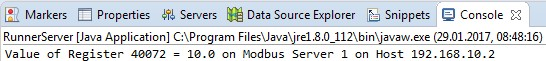
\includegraphics[width=14cm]{BilderAllgemein/pushServer1Ende.jpg}\medskip
 	\caption{Modbus Server VM1 nach dem Test}
 	\label{fig:PushAfterModbusServerVM1}
\end{figure}

\begin{figure}[h]
	\centering
	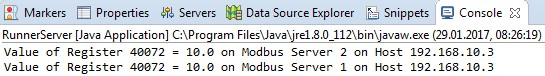
\includegraphics[width=14cm]{BilderAllgemein/pushServer2Ende.jpg}\medskip
 	\caption{Modbus Server VM2 nach dem Test}
 	\label{fig:PushAfterModbusServerVM2}
\end{figure}
\clearpage



\section{Request-Response (request)}

In diesem Kapitel wird der Test zum Validieren der implementierten Request-Response Funktion beschrieben.

\subsubsection{Ausgangssituation}
\label{sec:RequestResponseAusgangssituation}
Die Ausgangssituation der Request-Response Funktion ist dieselbe wie beim Test der Push Funktion, siehe Kapitel \ref{sec:PushAusgangssituation}. Für diesen Test wird nur der Modbus Server der VM1 benötigt. 

\subsection{Test}
Mit der \textit{request} Methode der \textit{ModbusTCPAdapter} Klasse wird nun ein Datenpunkt des Modbus Servers der VM1 ausgelesen. Listing \ref{lst:request} zeigt den Methodenaufruf. Der Methode wird der String im Format \textit{Remoteaddress} übergeben. Rückgegeben wir ein Objekt \textit{Result}. Bei diesen Test soll der SunSpec \textit{Float} Wert beginnend ab Register 40072 ausgelesen werden. Nach dem Aufruf der Methode wird das Rückgabeobjekt der Methode zu Testzwecken auf die Kommandozeile geschrieben. Hier soll auch der abgefragte Wert ausgegeben werden.


\lstset{language=Java, numbers=left, numberstyle=\tiny, stepnumber=2, numbersep=5pt, tabsize=2}
\begin{lstlisting}[caption={Methodenaufruf request},label=lst:request, xleftmargin=50pt]
public static void main(String[] args){
	//Neuer Adapter 
	ModbusTCPAdapter Adapter = ModbusTCPAdapter.getInstanz();
	//request response
	Result Feedback = new Result();
	try {
		Feedback = Adapter.request("192.168.10.2:1:40072:float32");
	} catch (Exception e) {
		// TODO Auto-generated catch block
		e.printStackTrace();
	}
	//Ausgabe der Antwort der Request-Response
	System.out.println(Feedback.data.data.toString());
	System.out.println(Feedback.status);
	System.out.println("Datentyp " + Feedback.data.datatype);
}
\end{lstlisting}
\clearpage

Tabelle \ref{tab:RequestRequestResponseFunktion} zeigt die Daten des TCP Segments der Modbus Anfrage an den Modbus Server der VM1. Der Aufbau des Modbus Frames wird im Kapitel \ref{sec:Protokollaufbau} beschrieben. Im folgenden Text wird dies anhand der aufgezeichneten Daten validiert. Die Felder des MBAP Headers sind bereits in Kapitel \ref{sec:Protokollaufbau} beschrieben. Als einziges soll hier das letzte Byte, die Slave ID im MBAP Header, betrachtet werden welches den Wert 1 hat. Diese stimmt mit jener überein, die der \textit{request} Methode übergeben wurde. Der im Kapitel \ref{sec:LeseHoldingRegisters} beschriebene Funktionscode 0x03 wurde durch die Modbus Library vergeben. Die Startadresse mit dem Wert 40072 stimmt mit dem Übergabeparameter der \textit{request} Methode überein. Es werden 2 Register für einen SunSpec \textit{Float} Wert benötigt. Auch dies wird in der Tabelle so dargestellt.

% Please add the following required packages to your document preamble:
% \usepackage{multirow}
\begin{table}[h]
\label{my-label}
\begin{tabular}{|c|c|c|l|l|}
\hline
\multicolumn{5}{|c|}{TCP Daten}                                                                                                                                                           \\ \hline
Byte & hex & Wert                   & Beschreibung                                                                                                         &                              \\ \hline
0    & 0   & \multirow{2}{*}{0}     & \multirow{2}{*}{\begin{tabular}[c]{@{}l@{}}Identifizierung der Modbus\\ Request / Response Transaktion\end{tabular}} & \multirow{7}{*}{MBAP Header} \\ \cline{1-2}
1    & 0   &                        &                                                                                                                      &                              \\ \cline{1-4}
2    & 0   & \multirow{2}{*}{0}     & \multirow{2}{*}{0 = Modbus Protokoll}                                                                                &                              \\ \cline{1-2}
3    & 0   &                        &                                                                                                                      &                              \\ \cline{1-4}
4    & 0   & \multirow{2}{*}{6}     & \multirow{2}{*}{Anzahl der daraufolgenden Byte}                                                                      &                              \\ \cline{1-2}
5    & 6   &                        &                                                                                                                      &                              \\ \cline{1-4}
6    & 1   & 1                      & Salve ID                                                                                                             &                              \\ \hline
7    & 3   &                        & Funktionscode                                                                                                        & \multirow{5}{*}{Data}        \\ \cline{1-4}
8    & 9C  & \multirow{2}{*}{40072} & \multirow{2}{*}{\begin{tabular}[c]{@{}l@{}}Start Register Adresse der\\ zu lesenden Daten\end{tabular}}              &                              \\ \cline{1-2}
9    & 88  &                        &                                                                                                                      &                              \\ \cline{1-4}
10   & 0   & \multirow{2}{*}{2}     & \multirow{2}{*}{\begin{tabular}[c]{@{}l@{}}Anzahl der Register\\ welche gelesen werden\end{tabular}}                 &                              \\ \cline{1-2}
11   & 2   &                        &                                                                                                                      &                              \\ \hline
\end{tabular}
\caption{Modbus Request der Request-Response Funktion}
\label{tab:RequestRequestResponseFunktion}
\end{table}
\clearpage

Tabelle \ref{tab:ResponseRequestResponseFunktion} stellt die Modbus Antwort des Modbus Servers der VM1 dar. Vergleicht man diese mit der zu erwartenden (siehe \ref{sec:LeseHoldingRegisters}) und der an den Server gesendeten Anfrage siehe Tabelle \ref{tab:RequestRequestResponseFunktion} kommt man zu folgenden Ergebnis. Es wird der an den Server gesendete  Funktionscode wieder zurückgesendet. Dies bedeutet die Modbus Transaktion war erfolgreich. Es wird die Anzahl an Werten zurückgesendet und die Werte in den Registern. Diese 4 Byte ergeben umgerechnet die Gleitkommazahl 1.1. Dieser Wert wird entsprechend Abbildung \ref{fig:PushBeforeModbusServerVM1} im Register dargestellt.

% Please add the following required packages to your document preamble:
% \usepackage{multirow}
\begin{table}[h]
\centering
\begin{tabular}{|c|c|c|l|l|}
\hline
\multicolumn{5}{|c|}{TCP Daten}                                                                                                                                                                                               \\ \hline
Byte & hex                     & Wert                 & Beschreibung                                                                                                                           &                              \\ \hline
0    & 0                       & \multirow{2}{*}{0}   & \multirow{2}{*}{\begin{tabular}[c]{@{}l@{}}Identifizierung der Modbus\\ Request / Response Transaktion\end{tabular}}                   & \multirow{7}{*}{MBAP Header} \\ \cline{1-2}
1    & 0                       &                      &                                                                                                                                        &                              \\ \cline{1-4}
2    & 0                       & \multirow{2}{*}{0}   & \multirow{2}{*}{0 = Modbus Protokoll}                                                                                                  &                              \\ \cline{1-2}
3    & 0                       &                      &                                                                                                                                        &                              \\ \cline{1-4}
4    & 0                       & \multirow{2}{*}{7}   & \multirow{2}{*}{Anzahl der darauffolgenden Byte}                                                                                        &                              \\ \cline{1-2}
5    & 7                       &                      &                                                                                                                                        &                              \\ \cline{1-4}
6    & 1                       & 1                    & Slave ID                                                                                                                               &                              \\ \hline
7    & 3                       & 3                    & Funktionscode                                                                                                                          & \multirow{6}{*}{Daten}       \\ \cline{1-4}
8    & 4                       & 4                    & Anzahl der Werte                                                                                                                       &                              \\ \cline{1-4}
9    & 3F                      & \multirow{4}{*}{1.1} & \multirow{4}{*}{\begin{tabular}[c]{@{}l@{}}Gelesene Register Werte:\\ Diese ergeben umgerechnet\\ die Gleitkommazahl 1.1\end{tabular}} &                              \\ \cline{1-2}
10   & 8C                      &                      &                                                                                                                                        &                              \\ \cline{1-2}
11   & CC                      &                      &                                                                                                                                        &                              \\ \cline{1-2}
12   & \multicolumn{1}{l|}{CD} &                      &                                                                                                                                        &                              \\ \hline
\end{tabular}
\caption{Modbus Response der Request-Response Funktion}
\label{tab:ResponseRequestResponseFunktion}
\end{table}
\clearpage

Im zweiten Testversuch der \textit{request} Methode wurde versucht, den Wert in einem Register des Modbus Servers der VM1 welches nicht vorhanden ist auszulesen. Tabelle \ref{tab:ResponseRequestResponseFunktionException} zeigt die Antwort des Modbus Servers. Der Funktionscode oder nun Errorcode besitzt den Wert 0x83. Dies entspricht dem zu erwartenden Code laut Modbus Standard. Als weiterer Wert wird noch ein Exceptioncode mitübertragen. Dieser besitzt den Wert 0x02 und entspricht ebenfalls der Modbus Spezifikation. 

% Please add the following required packages to your document preamble:
% \usepackage{multirow}
\begin{table}[h]
\begin{tabular}{|c|c|c|l|l|}
\hline
\multicolumn{5}{|c|}{TCP Daten}                                                                                                                                                       \\ \hline
Byte & hex & Wert               & Beschreibung                                                                                                         &                              \\ \hline
0    & 0   & \multirow{2}{*}{0} & \multirow{2}{*}{\begin{tabular}[c]{@{}l@{}}Identifizierung der Modbus\\ Request / Response Transaktion\end{tabular}} & \multirow{7}{*}{MBAP Header} \\ \cline{1-2}
1    & 0   &                    &                                                                                                                      &                              \\ \cline{1-4}
2    & 0   & \multirow{2}{*}{0} & \multirow{2}{*}{0 = Modbus Protokoll}                                                                                &                              \\ \cline{1-2}
3    & 0   &                    &                                                                                                                      &                              \\ \cline{1-4}
4    & 0   & \multirow{2}{*}{3} & \multirow{2}{*}{Anzahl der darauffolgenden Byte}                                                                      &                              \\ \cline{1-2}
5    & 3   &                    &                                                                                                                      &                              \\ \cline{1-4}
6    & 1   & 1                  & Slave ID                                                                                                             &                              \\ \hline
7    & 83  &                    & Funktionscode                                                                                                        & \multirow{2}{*}{Daten}       \\ \cline{1-4}
8    & 2   &                    & Exceptioncode                                                                                                       &                              \\ \hline
\end{tabular}
\centering
\caption{Fehlerhafte Modbus Response der Request-Response Funktion}
\label{tab:ResponseRequestResponseFunktionException}
\end{table}
